\documentclass[11pt, a4paper]{article}

\usepackage[utf8]{inputenc} 	% L'encodage. Ca peut être à remplacer par \usepackage[utf8]{inputenc}
\usepackage[T1]{fontenc}
\def\ques{\noindent{\bf Question : }}
\usepackage[english]{babel}
\usepackage[top=2cm, bottom=2cm, left=2cm, right=2cm]{geometry}		% Les marges
%\usepackage{listings}		% Pour mettre du code dans le fichier, il suffira ensuite d'appeler \begin{lstlisting}
%\lstset{
%language=Python,        	% choix du langage : C, Python, R, PHP...
%basicstyle=\footnotesize\color{mygray},       % taille de la police du code
%numbers=left,                   % placer les num�ros de lignes à droite (right) ou à gauche (left)
%numberstyle=\footnotesize,        % taille de la police des num�ros
%numbersep=7pt,                  % distance entre le code et sa num�rotation
%stepnumber=1,
%tabsize=4
%}
\usepackage{lscape}
\usepackage{amsthm}
\newtheorem{theorem}{Theorem}
\newtheorem{definition}{Definition}
\setcounter{theorem}{0}
\usepackage{comment} 
\usepackage{float}
%\usepackage{capt-of}
\usepackage{graphicx}	% Si besoin de bosser sur des images. Si besoin, aller sur le SDZ.
\usepackage{color}
\definecolor{mygray}{rgb}{0.2,0.2,0.2}
\usepackage{xcolor}
\usepackage{multicol}
% Les packages pour mettre des expressions un peu math�matis�es.
\usepackage{amsmath}
\usepackage{amssymb}
\usepackage{amsthm}
\usepackage{mathrsfs}
%\usepackage{mathtools}
%\usepackage{dsfont}
\newcommand{\horrule}[1]{\rule{\linewidth}{#1}}
\newcommand{\SR}[2]{\textcolor{gray}{#1}\textcolor{blue}{#2}}


\newtheorem{question}{Q}
\title{	
Composite likelihood inference of the parameters of a Poisson log-normal distribution
}

\date{\today}
\author{Elsa TEULIERE}

\graphicspath{ {./figures/} }
 

\begin{document}
\maketitle
\vspace{1cm}
\section*{Introduction}
\indent In ecology, studying a community of species often implies analysing correlated count data. Famous exemples are plant-polinisator or host-pathogens network studies. Ecologists often try to explain the effect of different covariates, for exemple climate in the case of plant-polinisators, or stress level for host-pathogens, on the interactions or, simply, abundance. The classical linear model will difficultly estimate this effect, since the counsidered species are highly dependent on each other. The response of one particular insect on climate change, will depend on the response of the species of plant it feeds on.\\

The Poisson log-normal Model (PLN-Model), developped by Aitchison \textit{et al.}\cite{aitchison1989multivariate} allows to take in account this dependency. The idea is to introduce a gaussian latent variable that will capture all the dependency in the network. Conditionally to this latent variable, the observed count variables will be independant and follow a Poisson distribution. Chiquet \textit{et al.} \cite{chiquet2017variational} proposed an estimation of the parameters of the Poisson log-normal distribution using a Variational Expectation-Minimization algorithm. However there exists no formal results on the consistency, nor on the asymptotic normality of this estimators. We were interested in constructing an consistent and asymptotically normal estimator of the parameters.\\

 We propose to estimate the parameters by maximizing a pairwise composite likelihood function. We show the consistency of this methode and give some tracks to proove the asymptotic normality of the estimator. \\ 

The report is organised as follow : after a short presentation of the PLN model,  we present, in a second part the composite likelihood and propose an estimator of the parameters of the Poisson log-normal model by maximizing it. We show this estimator to be consistent and expect it to be assymptotically normal. In a third part, we study the case of a structured dependency  and present the calculations in this case. Finally we present some simulations of the estimators. To conclude we propose an adaptation of the PLN model in order to take in account spatial dependencies. 

\section{Poisson log-normal model}
The Poisson log-normal model was developped by Aitchison \textit{et al.}\cite{aitchison1989multivariate}, to model multivariate count data.  The idea is to introduce gaussian latent variables encoding the dependency between the variables. In this section we introduce the model and our notations.
\subsection{Definitions and notations}
We note $\mathcal{N}_n (p,Q)$ the multivariate gaussian distribution in dimension $n$ of mean $p \in \mathbb{R}^n$ and variance-covariance $Q \in \mathcal{M}_n(\mathbb{R})$, and $\mathcal{P}(\alpha)$ the Poisson-distribution of mean $\alpha \in \mathbb{R}_+$.
\subsubsection{The Model} 
We consider $(\mu,\Sigma) \in \mathbb{R}^n \times \mathcal{M}_n(\mathbb{R})$, with $\Sigma$ a symetric non negative matrix, the parameters of the model. $\mu$ is the vector of mean and $\Sigma$ the matrix of variance-covariance.\\
We consider the latent variables $Z \sim \mathcal{N}_n(0,\Sigma)$.\\
Multivariate count data $(Y_1,...,Y_n)$ follow a Poisson log-normal distribution of mean $\mu$ and matrix of variance-covariance $\Sigma$ if :
\begin{center}
$\forall i \in \{1,...n\}, Y_i \mid Z_i \sim \mathcal{P}(e^{\mu_i+Z_i})$
\end{center}
and 
\begin{center}
$\forall (i,j) \in \{1,...,n\}^2$, $ Y_i\mid Z_i$ and $Y_j\mid Z_j$ independant.
\end{center}

We typically consider $N$ independant sampling experiment of $n$ variables each time, for example the case of sampling $n$ species over $N$ sites. In our notations, the exposant allways stands for the sampling experiment, and the underscore stand for the observed variable.\\
So we now have $(Z^j)_{j \in \mathbb{N}}$ latent variables, independant and identically distributed : $\forall j \in \{1,...,N\}$, $Z^j \sim \mathcal{N}_n(0,\Sigma)$, and :
\begin{center}
$\forall (i,j) \in \{1,...,n\} \times \{1,...,N\}$, $Y^j_i \mid Z^j_i \sim \mathcal{P}(e^{\mu_i+Z^j_i})$.
\end{center}
The advantage of this model is that all the dependance structure is encoded through gaussian variables.
\subsubsection{Extension accounting for covariates and offset}
In multivariate data, the dependency can occur through covariates. As developped in \cite{chiquet2017variational}, we will postulate the existence of a linear regression in  the parameters space. \\
\\
In this case, we consider a vector $X^j \in \mathbb{R}^d$ of covariates (collected for each sampling). Let $M$ be a $d \times n$ Matrix, called the matrix of regression parameters. We note $m^{(i)}$ the $i^{th}$ column of the matrix M. We can also add one offset parameter per observation : $O^j_i$. The offset, can typically be the sampling effort. In this case the Poisson log-normal model is given by :
\begin{center}
$\forall (i,j) \in \{1,...,n\} \times \{1,...,N\}$, $Y^j_i \mid Z^j_i \sim \mathcal{P}(e^{O^j_i + X_j^T \mu^i +Z^j_i})$ 
\end{center}
The set of parameters, that we aim to estimate is now given by $(M,\Sigma) \in \mathcal{M}_{d \times n}(\mathbb{R}) \times \mathcal{M}_{n}(\mathbb{R})$. $M$ is the matrix of regression parameter. Each column of $M$ contain all the regression parameters toward the covariables for one observed variable. We will now use the following notations : $X \in \mathcal{M}_{d \times N} ( \mathbb{R})$ stands for the matrix of covariates. The $j^{th}$ column of $X$ contains the covariates for the $j^{th}$ sampling. $O =(O_{ij}) \in \mathcal{M}_{n \times N} (\mathbb{R})$ stands for the matrix of offsets, we consider that $O_{ij}=O^j_i$. \\
\\
This model enable us to take in account for fixed additional effects. Indeed, it can help to interpret the dependency parameters. For examples, 	Poisson log-normal model can be used to estimate an interaction network from the co-occurances. With this model, we can hope, with a good choice of the covariates, that the dependencies encoded in the variance-covariance matrix $\Sigma$ will indicate the interraction between species.
\subsection{Properties}
\subsubsection{Density function of the Poisson log-normal distribution}
Following \cite{aitchison1989multivariate}, the Poisson log-normal distribution admits a density function given by :
\begin{center}
$\forall (y_1,...y_n) \in \mathbb{N}^n$, $h_{(\mu,\Sigma)}(y_1,...y_n)=\int_{\mathbb{R}^n} \prod_{i=1}^n f_{e^{\mu_i+z_i}}(y_i) g_{(0,\Sigma)}(z_1,...z_n) \mathrm{d}z_1...\mathrm{d}z_n$
\end{center}
Where $f_{\alpha}$ stands for the density function of a Poisson distribution with parameter $\alpha \in \mathbb{R}_+$, and $ g_{(0,\Sigma)}$ for the density function of a multivariate Normal distribution with parameters $(0,\Sigma)$.\\
\\
Taking in account covariates and offset, give the following distribution function :
\begin{center}
$ \forall X \in \mathbb{R}^d, \forall O \in \mathbb{R}^d, \forall (m_1,...m_n) \in \mathbb{N}^n$, $h_{(M,\Sigma \mid X, O)}(m_1,...m_n)=\int_{\mathbb{R}^n} \prod_{i=1}^n f_{e^{O_i+X^T \mu^i+z_i}}(m_i) g_{(0,\Sigma)}(z_1,...z_n) \mathrm{d}z_1...\mathrm{d}z_n$
\end{center}
\subsubsection{Moments of the Poisson log-normale distribution} Again, following \cite{aitchison1989multivariate}, the moments of the Poisson log-normale distribution can easily be obtained through conditional expectation. Considering the observation $Y^j_i$ is following a Poisson log-normal distribution with  parameters $(M , \Sigma)$ (with $\Sigma= (\sigma_{ij})$), the covariates $X \in \mathcal{M}_{d \times N} ( \mathbb{R})$ and the offset $O \in \mathcal{M}_{n \times N} (\mathbb{R})$ 
\begin{align*}
\mathbb{E}(Y^j_i)& =\mathrm{exp}(O_{ij}+ (X^j)^T\mu^i+\frac{1}{2}\sigma_{ii})\\
\mathbb{V}(Y^j_i)& =\mathrm{exp}(O_{ij}+(X^j)^T \mu^i+\frac{1}{2}\sigma_{ii})+(\mathrm{exp}(O_{ij}+(X^j)^T\mu^i+\frac{1}{2}\sigma_{ii})^2(\mathrm{exp}(\sigma_{ii})-1)\\
\mathrm{Cov}(Y^j_i,Y^j_k)& =\mathrm{exp}(O_{ij}+(X^j)^T \mu^i+\frac{1}{2}\sigma_{ii})\mathrm{exp}(O_{kj}+(X^j)^T \mu_k+\frac{1}{2}\sigma_{kk})(exp(\sigma_{ik}) - 1)
\end{align*}
\subsubsection{Overdispersion}
From the calculation of the moments, we see that for $Y^j_i$ following a Poisson log-normal distribution :
\begin{center}
$\mathbb{E}(Y^j_i) < \mathbb{V}(Y^j_i)$.   
\end{center}
The Poisson log-normal distribution is overdispersed, giving a clue that it can be applyed to a large range of multivariate count data, specially in ecology.
Indeed $\mathrm{Cov}(Y^j_i,Y^j_k)$ and $\sigma_{ik}$ have the same sign.\\
\\
The Poisson log-normal seems to be an appropriate model to study count data with a dependency structure. Furthermore this model as been already studied and in particular the Variational Estimation Minimization has been applied to it \cite{chiquet2017variational}. Although there exist no assymptotic guaranties on this estimation, our idea is to use this efficient estimation to initialize for the search for other estimators that can be computationally very costly.
\section{Composite likelihood estimation}
\subsection{Definition and notation}
\subsubsection{Presentation of the composite likelihood}
One classical method to estimate the parameters of a distribution is to maximize a so called likelihood-function over all the parameters sets. The likelihood-function is typically the density of the modelled distribution taken over all observations :
\begin{center}
$\mathcal{L}_{(Y^1,..Y^N)}(M,\Sigma \mid X,O) = \prod_{j=1}^N h_{(M,\Sigma \mid X,O)}(Y^j)$
\end{center}
When the considered density function is in the exponential family, the log-likelihood, expressed as follow, is more appropriated : 
$\mathcal{L}_{(Y^1,..Y^N)}(M,\Sigma \mid X,O) = \sum_{j=1}^N \mathrm{log} (h_{(M,\Sigma \mid X,O)}(Y^j))$.\\
\\ 
In our case, the likelihood function is costly to calculate, because the dependency structure in the data implies to calculate integrals over $\mathbb{R}^n$. Several approached have been proposed in order to symplify the likeiyhood function in the case of complex dependencies. We propose to use the composite likelihood approach (see\cite{varin2011overview}, \cite{pedeli2018pairwise} and \cite{varin2008composite}).\\
\\
Composite likelihood is expressed as a weighted product of the marginal or conditional density functions.
\begin{definition}\cite{varin2011overview} Let $Y$ be a $n$-dimensional random vector, with density function $f_\theta$ parametrized by a $p$-dimensional unknown parameter $\theta \in \Theta$.\\
Let $\{\mathcal{A}_1,..., \mathcal{A}_k\}$ be a set of marginal or conditional events. We note $\mathcal{L}^k_{(y)} (\theta) \varpropto f_\theta(y \in \mathcal{A}_k)$ the associated (marginal or conditional) likelihood. The composite likelihood is then given by :
\begin{align*}
\mathcal{CL}_{(y)}(\theta) = \prod_{i=1}^k (\mathcal{L}^i_{(y)}(\theta))^{w_i} 
\end{align*}
Where $w_i$ are non negative weights to be choosen.
\end{definition}
The idea behind composite marginal likelihood \cite{varin2008composite} is to compose low dimensional marginal densities in order to symplify the calculations, but also to capture the dependence between the parameters. \\
If there is no dependance structure, it is sufficient to take the product of the one-dimensional densities. Otherwise, at least, the two-dimensionnal marginal densities are needed  to capture the  dependence between the parameters.\\
\\
No theoretical results exist about the loss of efficiency \cite{lele2006sampling}. The idea is to show that maximizing the composite likelihood is a consitent assymptotic estimator of the parameters.

\subsubsection{Composite likelihood for the PLN model}
In our case, by integration, we can show that the two-dimensional marginal density function is given by $ \forall (m_1,m_2) \in \mathbb{N}^2$,$\forall X \in \mathbb{R}^d$, $ \forall O \in \mathbb{R}^d$ :
\begin{center}
 $\sum_{(m_3...m_n) \in \mathbb{N}^{n-2}} h_{(\mu,\Sigma \mid X)}(m_1,...m_n) = \int_{\mathbb{R}^2} f_{e^{O_1+X^T \mu^1+z_1}}(m_1) f_{e^{O_2+X^T \mu^2+z_2}}(m_2) g_{(0,\Sigma^{(12)})}(z_1,z_2)\mathrm{d}z_1 \mathrm{d}z_2$.
\end{center}
with $\Sigma^{(12)}=\begin{pmatrix}
\sigma_{11} & \sigma_{12} \\
\sigma_{12} & \sigma_{22}\\
\end{pmatrix}$\\
With this simple expression of the pairwise density function, we can write the composite pairwise marginal density function given by : $\forall (Y^1,...,Y^N) \in (\mathbb{R}^n)^N$, $\forall O \in \mathcal{M}_{n \times d} (\mathbb{R})$, $\forall X \in \mathcal{M}_{d \times N}(\mathbb{R})$ :
\begin{align}
\mathcal{CL}_{(Y^1,...,Y^N,O)}(M,\Sigma \mid X) = \prod_{j=1}^N \prod_{1 \leq i < k \leq n}  h'_{(M^{(ik)},\Sigma^{(ik)} \mid X^j,O^j)}(Y^j_i,Y^j_k)
\end{align}
With $h'$ the pairwise density function defined as above , $M^{(ik)}$ the matrix constituted of the $i$-th and $k$-th columns of M and 
$\Sigma^{(ik)}  = \begin{pmatrix}
\sigma_{ii} & \sigma_{ik}\\
\sigma_{ik} & \sigma_{kk}\\
\end{pmatrix}$
For easier calculation, we take the log composite likelihood given by :
\begin{align*}
\mathcal{CL}_{(Y^1,...,Y^N,O)}(M,\Sigma \mid X) = \sum_{j=1}^N \sum_{1 \leq i < k \leq n}  \mathrm{log}(h'_{(M^{(ik)},\Sigma^{(ik)} \mid X^j,O^j)}(Y^j_i,Y^j_k))
\end{align*}
 In the next section we show that the pairwise log-composite likelihood, is an M-estimator and so all the theory developped for M-estimators \cite{vaart_1998} can be applied.
\subsubsection{M-estimator and composite likelihood}
\begin{definition}
Let $(Y^1,...Y^N) \in \mathcal{X}^N$ be a set of observations. Let $\theta$ be an unknown parameter. \\
$\widehat{\theta}_N(Y^1,...Y^N)$ is called an M-estimator of $\theta$ if it maximize a function :
\begin{align*}
\mathcal{M}_N : \theta \mapsto \frac{1}{N} \sum_{i=1}^N m_\theta(Y^i)
\end{align*}
with, for all $\theta \in \Theta$, $m_\theta : \mathcal{X} \rightarrow \mathbb{R}$ a known function.
\end{definition}
Since the $\frac{1}{N}$ factor in the M-estimator does not modify the location of the maximum, we can also search for the maximum of an M-estimator by maximizing  $ \theta \mapsto  \sum_{i=1}^N m_\theta(Y^i)$.\\
\\
In the case of the composite likelihood, for all $\theta \in \Theta$, we set 
\begin{center}
$\begin{array}{ccccc}
m_\theta & : & \mathcal{X} & \to & \mathbb{R} \\
 & & Y^j & \mapsto & \sum_{0 \leq i<k \leq n} \mathrm{log} (h'_{(M^{(ik)},\Sigma^{(ik)})}(Y^j_i,Y^j_k) \\
\end{array}$
\end{center}
The estimator constructed by maximizing the pairwise composite likelihood is an M-estimator. We will apply the theory developped for M-estimators to prove the consistency and asymptotic normality of the estimator.
\subsection{Consistency}
\subsubsection{Consistency of M-estimators}
\begin{theorem} \label{ThMest} \cite{vaart_1998}
Let $(\mathrm{M}_N)$ be a random sequence of functions in the variable $\theta$ and $M$ a determinist function in the variable $\theta$. If :
\begin{enumerate}
\item $\underset{\theta \in \Theta}{\mathrm{sup}} \mid \mathrm{M}_N(\theta)-\mathrm{M}(\theta) \mid \overset{\mathbb{P}}{\longrightarrow} 0$
\item the maximum $\theta^\ast$ of M is unique.
\end{enumerate}
Then any sequence of estimators $\widehat{\theta}_N$ with $\mathrm{M}_N(\widehat{\theta}_N) \geq \mathrm{M}_N(\theta^\ast)-\circ_p(1)$ converges in probability to $\theta^\ast$.
\end{theorem}
\begin{proof}
Let $M_N$ a random sequence of function, $M$ a determinist function with a unique maximum $\theta^*$ and $\widehat{\theta}_N$ be a sequence of estimators satisfying the conditions of the theorem \ref{ThMest}.

We want to proove that :
\begin{center}
$\forall \epsilon > 0$, $\mathbb{P}(\{\mathrm{d}(\widehat{\theta}_N,\theta*)>\epsilon\})\underset{ N \rightarrow + \infty}{\longrightarrow} 0$
\end{center}
Let consider $\epsilon >0$. By assumption, $\theta ^*$ is the unique maximum of the function $M$, so $\underset{ \theta : \mathrm{d}(\theta,\theta^*)}{\mathrm{sup}}(M(\theta)) < M(\theta^*)$. In particular, there exists $\eta > 0$ so that : $\forall \theta \in \Theta$, $\mathrm{d}(\theta,\theta^*)>\epsilon$, $M(\theta) < M(\theta^*)-\eta$.\\
Consequently, the probabilist event $\{\mathrm{d}(\widehat{\theta}_N,\theta^*)> \epsilon\}$ is included in the event $\{M(\widehat{\theta}_N)<M(\theta^*)-\eta\}$. We will show that the probability of this event converges to zero when $N$ tends to infinity.\\
The assumption of uniform convergence of the sequence of functions $M_N$  to $M$ ensures that $M_N(\theta^*) \overset{\mathbb{P}}{\longrightarrow} M(\theta^*)$. Indeed, by assumption $M_N( \widehat{\theta}_N) \geq M_N(\theta^*)- \circ_\mathbb{P}(1)$, so we deduce that $M_N( \widehat{\theta}_N)+ \circ_\mathbb{P}(1) \geq M(\theta^*)$.
We now deduce that :
\begin{align*}
M(\theta^*)-M(\widehat{\theta}_N) & \leq \widehat{\theta}_N)+ \circ_\mathbb{P}(1)-M(\widehat{\theta}_N)\\
& \leq \underset{\theta}{\mathrm{sup}} \mid M_N-M \mid (\theta) + \circ_\mathbb{P}(1)
\end{align*}
This is sufficient to conclude since for all $\eta > 0$, $\mathbb{P} ( \mid M(\theta^*)-M(\widehat{\theta}_N)\mid > \eta) \underset{ N \rightarrow + \infty} {\longrightarrow} 0$.
\end{proof}
\subsubsection{Consistency of the composite likelihood for the PLN model}
The estimator of the parameters $M$ and $\Sigma$ of a Poisson log-normal model constructed by maximizing the composite likelihood is consistent. We show this result in two steps. We first show that for a Poisson log-normal model in dimension two, the maximum-likelihood estimator is consistent before generalizing to $n$-dimensional PLN models.

\paragraph{In dimension 2} :
\begin{theorem} \label{Consistence_2}
For each $(i,k) \in \{1...n\}^2$, $i \neq k$, the estimator $(\widehat{M}^{(ik)}_N,\widehat{\Sigma}^{(ik)}_N)$ constructed by maximizing the log-likelihood of the couple $(Y^j_i,Y^j_k)_{j \in \{1...N\}}$, given by $\sum_{i=1}^{N} \mathrm{log}(p_{(M^{(ik)},\Sigma^{ik} \mid X)}(Y^j_i,Y^j_k))$, is a consistent estimator of the regression coefficients $M^{(ik)}$ and of the variance-covariance matrix $\Sigma^{(ik)}$.
\end{theorem}
\begin{proof}

The idea of the proof is to use the theorem \ref{ThMest} for the pairwise composite likelihood. The proof will  follow four steps to verify that the assumptions of the theorem are verified. We will first show the convergence in probability of our M-estimator to a function $\mathcal{M}{(M^{(ik)},\Sigma^{(ik)})}$. Then we proove the existence of a unique maximum for this function $\mathcal{M}$. We proove this, we  first  show that our model is identifiable. Then, using the Kullback-divergence, we show that it has a  maximum. Combining this two steps will allow us to conclude the existence of a unique maximum. In the last part, we conclude, using the theroem \ref{ThMest} on the consistence of the estimator. \\
\\
\textbf{Step 1 :} Convergence in probability.\\
Using the large number law, we do have that $\frac{1}{N} \sum_{i=1}^{N} \mathrm{log}(h_{(M^{(ik)},\Sigma^{(ik)} \mid X)}(Y^j_i,Y^j_k))$ converge almost surely to $\mathbb{E}_X[\mathbb{E}_{Y_i Y_k \mid X}[ \mathrm{log}(h_{(M^{(ik)},\Sigma^{(ik)} \mid X)}(Y_i,Y_k))]]$.\\
 So we set $\mathcal{M}(M^{(ik)}, \Sigma^{(ik)}) =\mathbb{E}_X[\mathbb{E}_{Y_i Y_k \mid X}[ \mathrm{log}(h_{(M^{(ik)},\Sigma^{(ik)} \mid X)}(Y_i,Y_k))]]$. \\
\\
\textbf{Step 2 :} Identifiability of the model.\\
 We use the general definition of identifiability \cite{rivoirard}, namely that the family of probabilities $\mathcal{P}=\{\mathbb{P}_\theta,\theta \in \Theta\}$ is identifiable if the application $ \theta \mapsto \mathbb{P}_\theta$ is injective.
 In our case $\mathcal{P}=\{(\mathcal{PLN}_X (M,\Sigma))_{X \in \mathcal{X}}; (\mu, \Sigma) \in  \mathcal{M}_{d \times n}(\mathbb{R}) \times \mathcal{M}_n(\mathbb{R})\}$. To show the identifiability of the model we will use the fact that two variables having the same distribution have the same moment. Consider $(M^{(ik)},\Sigma^{(ik)}) \in \mathcal{M}_{d\times 2}(\mathbb{R}) \times \mathcal{M}_2(\mathbb{R})$ and $(M'^{(ik)},\Sigma'^{(ik)}) \in \mathcal{M}_{d\times 2}(\mathbb{R}) \times \mathcal{M}_2(\mathbb{R})$, so that  for every vector of covariates $X \in \mathcal{X}$,$\mathcal{PLN}_X(M^{(ik)},\Sigma^{(ik)})\sim\mathcal{PLN}_X(M'^{(ik)},\Sigma'^{(ik)})$ . We have :
 \begin{equation}
 \mathbb{E}_{(M^{(ik)},\Sigma^{(ik)} \mid X)}[Y_i]=\mathbb{E}_{(M'^{(ik)},\Sigma'^{(ik)} \mid X)} [Y_i] 
 \end{equation}
\begin{equation}
 \mathrm{Var}_{(M^{(ik)},\Sigma^{(ik)} \mid X)}[Y_i]=\mathrm{Var}_{(M'^{(ik)},\Sigma'^{(ik)} \mid X)} [Y_i] \\
\end{equation}
\begin{equation}
 \mathrm{Cov}_{(\mu^{(ik)},\Sigma^{(ik)} \mid X)}[Y_i,Y_k]=\mathrm{Cov}_{(M'^{(ik)},\Sigma'^{(ik)} \mid X)} [Y_i,Y_k]
\end{equation}
Using the formula of this moment we recall in the presentation of the model, we find that $\sigma_{ii} = \sigma'_{ii}$, $\sigma_{ik}=\sigma'_{ik}$ and $X (M^i-M'^i)=0$. The last condition has to be true for any vector of covariable $X$. We deduce from this that,  we expect $\mathcal{X}^\perp = \{0\}$ for the model to be identifable, \textit{ie.} that $\mathrm{rg}(\mathcal{X})=d$.\\
\\
\textbf{Step 3 :} Existence of a unique maximum for the function $\mathrm{M}$.\\
What we consider is nothing else than the log-likelihood of two variables with a Poisson-log-normale distribution. We just shew that the model is identifiable. So there exist one and only one set of parameters $(M^{(ik)\ast}, \Sigma^{(ik)\ast})$ such that $(Y_i,Y_k) \sim \mathcal{PLN}_X(M^{(ik)\ast},\Sigma^{(ik)\ast})$. We first can show that maximizing the log-likelihood is equivalent to minimize the Kullback divergence. We recall that the Kullback divergence for two distributions of density functions $p_\theta$ and $p_{\theta^\ast}$ is given by $\mathrm{D_{KL}}(p_{\theta^\ast} \parallel p_{\theta})= \int p_{\theta^\ast}(x) \mathrm{log}(\frac{p_{\theta^\ast}(x)}{p_{\theta}(x)}) \mathrm{d}x$. Since we have :
\begin{align*}
\mathbb{E}_X[\mathbb{E}_{(M^{(ik)\ast},\Sigma^{(ik)\ast} \mid X)}&[\mathrm{log}(h_{(M^{(ik)\ast},\Sigma^{(ik)\ast} \mid X)}(Y_i,Y_k)) - \mathrm{log}(h_{(M^{(ik)},\Sigma^{(ik)} \mid X)}(Y_j,Y_k))]] \\
& = \mathbb{E}_X[\mathrm{D_{KL}}(h_{(\mu_{jk}^\ast,\Sigma_{jk}^\ast \mid X)}\parallel h_{(\mu^{(ik)},\Sigma^{(ik)} \mid X)})]\\
& = \mathbb{E}_X[\mathbb{E}_{(M^{(ik)\ast}\,\Sigma^{(ik)\ast} \mid X)}[\mathrm{log}(h_{(M^{(ik)\ast},\Sigma^{(ik)\ast} \mid X)}(Y_i,Y_k))]] - \mathrm{M}(M^{(ik)},\Sigma^{(ik)})
\end{align*}
 Since the Kullback-divergence is always positive, we see that maximizing the log-likelihood is equivalent to minimize the Kullback-divergence. The Kullback-divergence is only zero if the two distributions are the same. So we see that the $\mathcal{M}$ function is maximum for $(M^{(ik)},\Sigma^{(ik)})=(M^{(ik)\ast},\Sigma^{(ik)\ast})$. This conclude. The function $\mathcal{M}$ only has one maximum, and this maximum is obtained for the parameters we are interested in.\\
\\
\textbf{Step 4 :} Conclusion.\\
To summurize we have :
\begin{enumerate}
\item By the convergence almost surely :
\begin{center}
 $\underset{(M^{(ik)},\Sigma^{(ik)})}{\mathrm{sup}} \mid \frac{1}{N} \sum_{j=1}^{N} \mathrm{log}(h_{(M^{(ik)},\Sigma^{(ik)} \mid X)}(Y^j_i,Y^j_k)) - \mathbb{E}_X[\mathbb{E}_{Y_i Y_k \mid X}[\mathrm{log}(h_{(M^{(ik)},\Sigma^{(ik)} \mid X)}(Y_i,Y_k))]] \mid$\\ $\overset{\mathbb{P}}{\longrightarrow} 0 $ 
 \end{center}
\item The function $(M^{(ik)},\Sigma^{(ik)})\mapsto \mathbb{E}_X[\mathbb{E}_{Y_i Y_k \mid X}[\mathrm{log}(h_{(M^{(ik)},\Sigma^{(ik)} \mid X)}(Y_i,Y_k))]] $ only has one maximum for $(M^{ik},\Sigma^{(ik)})=(M^{(ik)\ast},\Sigma^{(ik)\ast})$, the parameters of the Poisson-log-Normale distribution of the variables $(Y_i,Y_k)$.
\item We note $\mathcal{M}_N$ the pairwise likelihood over N observations. Then $\mathcal{M}_N(\widehat{M}^{(ik)}_N,\widehat{\Sigma}^{(ik)}_N) \geq \mathcal{M}_N(M^{(ik)\ast},\Sigma^{(ik)\ast}) $.
\end{enumerate}
Applying theorem \ref{ThMest}, we conclude that the sequence of estimators $(\widehat{M}^{(ik)}_N, \widehat{\Sigma}^{ik}_N)_{N \in \mathbb{N}}$ converges in probability to what we hope to approximate, namely $(M^{(ik)\ast}, \Sigma^{(ik)\ast}$).
\end{proof}

\paragraph{In dimension $n$}
\begin{theorem}
The estimator $(\widehat{M}_N,\widehat{\Sigma}_N)$ constructed by maximizing the composite pairwise likelihood for $(Y^j_1,...Y^j_n)_{j \in \{1...N\}}$ is a consistent estimator of the correlation coefficients $M$ and of the matrix of variance-covariance $\Sigma$.
\end{theorem}

\begin{proof}
The proof follows exactly the same path that for a couple of variables. We will again use theorem \ref{ThMest} and the results of theorem \ref{Consistence_2}.\\
\\
\textbf{Step 1 :} Convergence in probability.
Again using the large number law we have :\\
 $\frac{1}{N}\sum_{i=1}^{N} \sum_{j<k} log(h_{(M^{(ik)},\Sigma^{(ik)} \mid X)} (Y^j_i,Y^j_k) \overset{\mathbb{P}}{\longrightarrow} \sum_{j<k}\mathbb{E}_X [\mathbb{E}_{Y_i Y_k \mid X}[\mathrm{log}(h_{(M^{(ik)},\Sigma^{(ik)} \mid X)}(Y_i,Y_k))]]$.\\
 We note M the function $\mathrm{M} : (M, \Sigma) \mapsto \sum_{j<k}\mathbb{E}_X [\mathbb{E}_{Y_i Y_k \mid X}[\mathrm{log}(h_{(M^{(ik)},\Sigma^{(ik)} \mid X)}(Y_i,Y_k))]]$.\\
 \\
 \textbf{Step 2 :} Identifiability of the model.\\
The family of model we consider here is $\mathcal{P}=\{ (\mathcal{PLN}_X(\mu,\Sigma))_{X \in \mathcal{X}}; M \in \mathcal{M}_{d \times n}(\mathbb{R}), \Sigma \in \mathcal{M}_n(\mathbb{R})\}$. Using the moment as we did with a Poisson log-normal distribution of a vector of two variables, but this time for n variables is sufficient to show the identifiability of the model.\\
\\
\textbf{Step 3 :} Existence and uniqueness of the maximum for the function M.\\
Again here we have by the identifiability of the model, under the assumption that the data follow a Poisson log-normal distribution, that there exist one and only one set of parameters $(M^\ast, \Sigma^\ast)$ such as given a vector of covariates $X$, $(Y^j) \sim \mathcal{PLN}_X (M^\ast, \Sigma^\ast)$. As we did in the previous section we show that maximizing M is equivalent to minimize the function :\\
$(M, \Sigma) \mapsto \sum_{j<k} \mathbb{E}_X [\mathrm{D_{KL}}(h_{(M^{(ik)\ast},\Sigma^{(ik)\ast} \mid X)} \parallel h_{(M^{(ik)},\Sigma^{(ik)} \mid X)}]$.\\
We have here a finite sum of positive variables, so in order to minimize it, we can minimize each of the terms. Consequently the above function is minimal for $M^\ast=(M^{(i)\ast})_{i \in \{1...n\}}$ and $\Sigma^\ast$ defined as follow : the term $(\sigma_{ik})_{i \neq k}$ of $\Sigma^\ast$ is the term $\sigma_{12}$ of $\Sigma^{(ik)\ast}$  and the term $\sigma_{ii}$ of $\Sigma^\ast$ is the term $\sigma_{11}$ of $\Sigma^{(ik)\ast}$.\\
Thus we have the existence of a maximum and its uniqueness.\\
\\
\textbf{Step 4 :} Conclusion.\\
Applying theorem \ref{ThMest}, we conclude that the sequence of estimators $(\widehat{M}_N, \widehat{\Sigma}_N)_{N \in \mathbb{N}}$ maximizing the composite likelihood function $(M,\Sigma) \mapsto \mathcal{CL}_{(M,\Sigma) \mid X}((Y^j)_{j \in \{1..N\}})$  converges in probability to what we hope to approximate, namely $(M^\ast, \Sigma^\ast)$, the parameters of the Poisson log-normal model.
\end{proof}
\subsubsection{Estimation of the maximum.}
In order to estimate the maximum of the composite pairwise likelihood we performed an optimization algorithm. We  performed simulations to estimate the parameters.\\
The calculation of the density function of the Poisson log-normale distribution are quite costly to calculate. Since the optimization require calculation of the density function, we propose to initialize the optimisation algorithm with the results of the VEM for the Poisson log-normal model.
\subsection{Asymptotic normality}
The asymptotic normality is needed to construct asymptotic confidence sets and so statistic tests.
\subsubsection{M-estimator theory}
We define :
\begin{center}
$\Psi_n(\theta)=\frac{1}{N}\sum_{i=1}^N \Psi_\theta(X_i) = \mathbb{P}_N \Psi_\theta$\\
$\Psi(\theta) = \mathrm{P}\Psi_\theta$
\end{center}
\begin{theorem} \cite{vaart_1998} \label{ThAN}
Let $\Theta$ be an euclidian space. For each $\theta \in \Theta$, let $\theta \mapsto \Psi_\theta (x)$ une fonction $\mathcal{C}^2$ with respect to the variable $x$. Suppose that there exists $\theta_0$, such that $\mathrm{P} \Psi_{\theta_0} =0 $ and $\mathrm{P} \parallel \Psi_{\theta_0} \parallel^2 < \infty$. Indeed, we suppose that the matrix $\mathrm{P} \dot{\Psi}_{\theta_0}$ exists and is non-singular. Assume that the second-order partial derivatives are dominated by a fixed integrable function in the variable  $\ddot{\Psi}$ for every $\theta$ in a neiborhood of $\theta_0$. Consider a consistent estimator sequence $\widehat{\theta}_N$ such that $\Psi_N(\widehat{\theta}_N)=0$, the sequence $\sqrt{n}(\widehat{\theta}_N - \theta_0)$ converges in law to $\mathcal{N}(0,(\mathrm{P} \dot{\Psi}_{\theta_0})^{-1} \mathrm{P} \Psi_{\theta_0} \mathrm{P} \Psi_{\theta_0}^T (\mathrm{P} \dot{\Psi}_{\theta_0})^{-1}))$.
\end{theorem}
\subsubsection{Asymptotic normality of the composite likelihood for the PLN model}
We want to apply theorem \ref{ThAN} to our problem of M-maximization. In this case the function $\Psi_\theta$ is given by the derivative of the composite likelihood.\\
\\
We did not do the rigourous proof of this result, and we present here some tracks we explored to show this result.
At first, we see that the composite likelihood $(M,\Sigma) \mapsto \mathcal{CL}_{(Y^1,...,Y^N,O)}(M,\Sigma \mid X)$ function is three time continuously differentiable with respect to the variable $(M,\Sigma)$ for every $(Y^1,...,Y^N,O)$, because it is just the sum of the composition of three time continuously derivable functions.\\
We shew, for the consistency of the estimator, that there exists an unique maximum $(M^*,\Sigma^*)$ for the composite likelihood. We have to show, in order to apply theorem \ref{ThAN}, that :
\begin{enumerate}
\item the norm of the first order derivative of the composite likelihood with respect to the parameters $(M,\Sigma)$ admits a first order  moment (with respect to the observation) when taken at the value $(M ^*,\Sigma^*)$. 
\item the second order derivative of the composite likelihood with respect to the parameters $(M,\Sigma)$ admits a first order moment (with respect to the observtions) when taken at the value $(M^*,\Sigma^*)$. The obtained matrix has to be non singular.
\item the expectation (with respect to te observations) of the third order derivative of the $\mathcal{CL}$ is dominated in a neighborhood of $(M^*,\Sigma^*)$ by a function integrable over $\mathbb{R}^n$.
\end{enumerate}

We performed explicit calculation of the gradient and the hessian matrix of the pairwise composite likelihood in the case of the PLN-Model \ref{appendix}.\\
\\
 We give here an alternative expression of the derivatives of the composite likelihood with respect to the parameters, in order to estimate easily, and more generally the derivates. We write the calculus for one couple of observations $(Y_i,Y_j)$.
 \begin{align*}
 \mathrm{log}(h_{(M^{(ij)},\Sigma^{(ij)}} (Y_i,Y_j)) =\mathbb{E}_{Z_{(ij)}} [\mathrm{log} (f_{e^{X^TM^{(j)}+Z_j}}(Y_j)) + \mathrm{log}(f_{e^{X^TM^{(i)}+Z_i}} (Y_i) ) ]
 \end{align*}
In this way the only dependance in $\Sigma$ is expressed throught the mean with respect to the latent variable $Z$ and the only dependance in $M$ is in the density function of the Poisson distribution.\\
In order to derivate, we use the following mathematical fact : $\partial_x g(x) = g(x) \partial_x \mathrm{log}(g(x))$. Splitting the dependency in the variables, we get :
\begin{align*}
\partial_{M^{(ij)}} \mathrm{log}(h_{(M^{(ij)},\Sigma^{(ij)}} (Y_i,Y_j)) = \mathbb{E}_{Z_{(ij)}} [\partial_{(M^{(ij)}} \mathrm{log} (f_{e^{X^TM^{(j)}+Z_j}}(Y_j)) ] + \mathbb{E}_{Z_{(ij)}}[ \partial_{(M^{(ij)}} \mathrm{log}(f_{e^{X^TM^{(i)}+Z_i}} (Y_i) ) ]\\
\partial_{\Sigma^{(ij)}} \mathrm{log}(h_{(M^{(ij)},\Sigma^{(ij)}} (Y_i,Y_j)) = \mathbb{E}_{Z_{(ij)}} [( \mathrm{log} (f_{e^{X^TM^{(j)}+Z_j}}(Y_j)) +  \mathrm{log}(f_{e^{X^TM^{(i)}+Z_i}} (Y_i) ) ) \partial_{\Sigma^{(ij)}} \mathrm{log} (g_{(0,\Sigma^{(ij)})} (Z_{(ij)})) ]
\end{align*}
For the derivatives with respect to the regression parameters, the calculation of the derivative are done in the appendix (see \ref{grad}).
We get : 
\begin{align*}
\partial_{M^{(ij)}} \mathrm{log}(h_{(M^{(ij)},\Sigma^{(ij)}} (Y_i,Y_j)) = & \mathbb{E}_{Z_{(ij)}} [ X \frac{Y_j f_{e^{X^TM^{(j)}+Z_j}}(Y_j) - (Y_j+1) f_{e^{X^TM^{(j)}+Z_j}}(Y_j+1) }{f_{e^{X^TM^{(j)}+Z_j}}(Y_j)} ] \\
& + \mathbb{E}_{Z_{(ij)}} [ X \frac{Y_i f_{e^{X^TM^{(i)}+Z_i}}(Y_i) - (Y_i+1) f_{e^{X^TM^{(i)}+Z_i}}(Y_i+1) }{f_{e^{X^TM^{(i)}+Z_i}}(Y_i)} ]
\end{align*} 
\\
About the derivatives with respect to $ \Sigma$, note that
\begin{center}
$\mathrm{log} (g_{(0,\Sigma^{(ij)})} (Z_{(ij)})) = -\mathrm{log} (2 \pi \sqrt{\mathrm{det}(\Sigma^{(ij)}}) - \frac{1}{2} Z_{ij}^T \Sigma ^{-1} Z_{ij}$.
\end{center} 
Thanks to the formula given in \cite{petersen2008matrix}, we deduce that :
\begin{align*}
\partial_{\Sigma^{(ij)} } \mathrm{log} (\sqrt{\mathrm{det} \Sigma^{(ij)}}) = - ((\Sigma^{(ij)})^{-1})\\
\partial_{\Sigma^{(ij)} } (- \frac{1}{2} Z_{ij}^T \Sigma^{-1} Z_{ij} ) = \frac{1}{2} \Sigma^{-1} Z_{ij} Z_{ij}^T \Sigma^{-1}
\end{align*}
Putting it back into the expression of the derivative with respect to $\Sigma ^{(ij)}$, one have :
\begin{align*}
\partial_{\Sigma^{(ij)}} \mathrm{log}(h_{(M^{(ij)},\Sigma^{(ij)}} (Y_i,Y_j)) = & \mathbb{E}_{Z^{(ij)}} [ - (\Sigma^{(ij)})^{-1} ( \mathrm{log} (f_{e^{X^TM^{(j)}+Z_j}}(Y_j)) +  \mathrm{log}(f_{e^{X^TM^{(i)}+Z_i}} (Y_i) ) ) ] \\
& + \mathbb{E}_{Z^{(ij)}} [\frac{1}{2} \Sigma^{-1} Z_{ij} Z_{ij}^T \Sigma^{-1} ( \mathrm{log} (f_{e^{X^TM^{(j)}+Z_j}}(Y_j)) +  \mathrm{log}(f_{e^{X^TM^{(i)}+Z_i}} (Y_i) ) )]
\end{align*}
Because of lack of time we did not push forward the proof.\\
\\
In the simulations, we normalized the estimators by removing the true parameter and dividing by an estimation of the Godambe Matrix obtained by the empirical mean over the observations of the value obtained by the direct calculations (see \ref{appendix} and \ref{plot}).
\section{Composite likelihood inference for datawith a structured dependence}
\subsection{Poisson log-normal model in case of a structured variance convariance matrix}
Suppose that you have information of the dependency structure between the observed variables.This can typically be the case when studying genetic variants in a population. Phylogenetic \cite{pavoine2008testing} or genetic distance \cite{NEI2001828} can be calculated between individuals. In this case, and inspired by what is done in spatial model, we can assume that the dependance matrix is structured. We study here one exemple of structured dependency.
\subsubsection{Parametrisation of the PLN distribution in case of a structured dependence}
We introduce the following notations : 
\begin{itemize}
\item $n \in \mathbb{N}$ is the number of observed variables. We note $Y_1...Y_n$ the variables of interest.
\item $N \in \mathbb{N}$ represents the number of independant repetitions. For example the number of sampling. As previously, $X \in \mathcal{M}_{d \times N}(\mathbb{R})$ is the matrix of covariates.
\item We suppose the matrix of variance covariance to be structured in the form 
\begin{align*}
\Sigma = \sigma^2 \begin{pmatrix}
1 &  e^{-\alpha d_{1,2}} &  e^{-\alpha d_{1,2}} & \ldots &  e^{- \alpha d_{1,n}}  \\
 e^{-\alpha d_{1,2}} & 1 & \ldots & \ldots &  e^{- \alpha d_{2,n}}\\
 \vdots & & \ddots & & \vdots\\
 \vdots & & & \ddots & \vdots \\
 e^{-\alpha d_{1,n}} &  e^{-\alpha d_{2,n}} & \ldots & \ldots & 1 
\end{pmatrix}
\end{align*} 
with $d_{ij}$ the, for example; phylogenetic distance between the species $i$ and $j$, $\alpha$ the range, and $\sigma^2$ the variance.
\end{itemize}
 
 In case of a "structured" PLN, the number of parameters is reduce, since we only need to estimate $\sigma^2$ and $\alpha$ to capture the whole dependency structure. In a sense, there is more constraint in the matrix of variance and covariance.
\subsection{Estimation of the parameters for the model spatial}
\subsubsection{Explicit calculation of the gradient}
In \ref{spatial} we get explicit formula of what we obtained when calculating the derivatives with respect to $\alpha$ and $\sigma^2$ of one term of the composite likelihood, namely $\mathrm{log}(h_{(M^{(ij)},\alpha, \sigma^2)}$. We failed to explicitly calculate this term. In turns, we could propose to estimate this quantity using  numerical approximations such as Monte-Carlo Markov Chain algorithms.\\
\\
An other approach we tried, is to use an optimisation algorithms that do not need an explicit expression of the gradient. Different algorithms are implemented in the software \texttt{R} and some of them (we used \texttt{optim}) give an approximation of the hessian matrix at the optimum. This enabled us to use the asymptotic normality to construct confidence sets.
\subsubsection{Computational optimisation by using a sparse composite likelihood} \label{sparse}
The pairwise composite likelihood evaluation requires to the evaluation of $n^2$ Poisson log-normal density function. The evaluation of this function is computationally quite costly, since it implies to estimate an integral over $\mathbb{R}^2$. We propose an approach in order to limit the number of pairs taken in account in the composite likelihood, tipycally for the case of large datasets. \\
\\
Let consider $I$ a subset of $\{(i,j) \in \{1...n\}^2\}$. We define $\mathcal{CL}^I = \sum_{(i,j) \in I} \mathrm{log}( h_{(M^{(ij)},\alpha,\sigma^2)}(Y_i,Y_j)) $.The question is, how to choose an optimal subset $I$.\\
\\
The first constraint we have, is that each $i \in \{1...n\}$ has to appear at least once in $I$, in order to be able to estimate all the regression parameters.\\
\\
We get the second constraint from the linear regression of the covariances and the distance between the species or individuals.
Note $\widehat{\sigma_{ij}}$ an estimator of the parameter of covariance $\sigma_{ij}$.
One have, by a linear model :
\begin{align*}
\mathrm{log}(\widehat{\sigma_{ij}}) = \mathrm{log} ( \sigma^2) - \alpha d_{ij} + E_{ij}
\end{align*}
With $E_{ij}$ a noise due to estimation. We estime this noise to be  independant and identically distributed  for all the considered couples. By a classical results for the linear regression model \cite{daudin1999statistique}, one have :
\begin{center}
$\mathbb{V}(\widehat{\alpha}) = \rho^2 (\frac{1}{n^2} + \frac{\bar{d}^2}{\sum_{(i,j)\in \{1..n\}^2}(d_ij - \bar{d})^2})$
\end{center}
Where $\rho^2$ is the variance of the error. We want to minimize the variance of $\widehat{\alpha}$. So we will try to maximize the quantity $\sum_{(i,j)\in \{1..n\}^2}(d_{ij} - \bar{d})^2$. This is our second constraint.\\
\\
Choosing $I$ under this two constraints, that is actually determining a maximum spanning tree over the following network : the vertices are the points $ \{i \in \{1...n\} \}$ and the edge between $i$ and $j$ is given by $d_{ij}$. We propose to choose the maximum spanning tree by using the Kruskal algorithm \cite{Kruskal1956}. 

\section{Simulations}
We performed simulation in order to illustrate our model.
\subsection{Implementation}
We implemented an algorithm in order to estimate the parameters of a Poisson log-normal distribution by maximizing the composite likelihood. The idea is the following.
\begin{enumerate}
\item We first performed a PLN model on the data, to get a first estimate of the parameters that we expect to be close to the solution. 
\item Using the nloptr package on \texttt{R} and the \texttt{NLOPT GN DIRECT L} algorithm we determined the parameters maximizing the composite pairwise likelihood. We optimized the pariwise composite likelihood under the constraint that the variance-covariance matrix is non negative.  The constraint function is thus :
\begin{align*}
f : \Sigma \mapsto - \mathrm{min}\{\lambda, \lambda \in Sp(\Sigma)\}
\end{align*}
We use an algorithm that doesn't need the explicit expression of the gradient (calculated in \ref{grad}), since we were not able, to calculate the gradient of the constraint. We set the default parameters of the \texttt{nlopt} function.
\item Then we estimated the Godambe matrix by the empirical mean of the value of the hessian taken over the observations. This calculation allows us to normalize the estimators.
\end{enumerate}

\subsection{Simulations}
We performed simulations in order to illustrate our results. We focus on the case of $N=100$ observations with $n=5$ variables of interest and $p=3$ covariates. The simulations were run over 250 repetitions. 
\begin{figure}[!h] \label{plot}
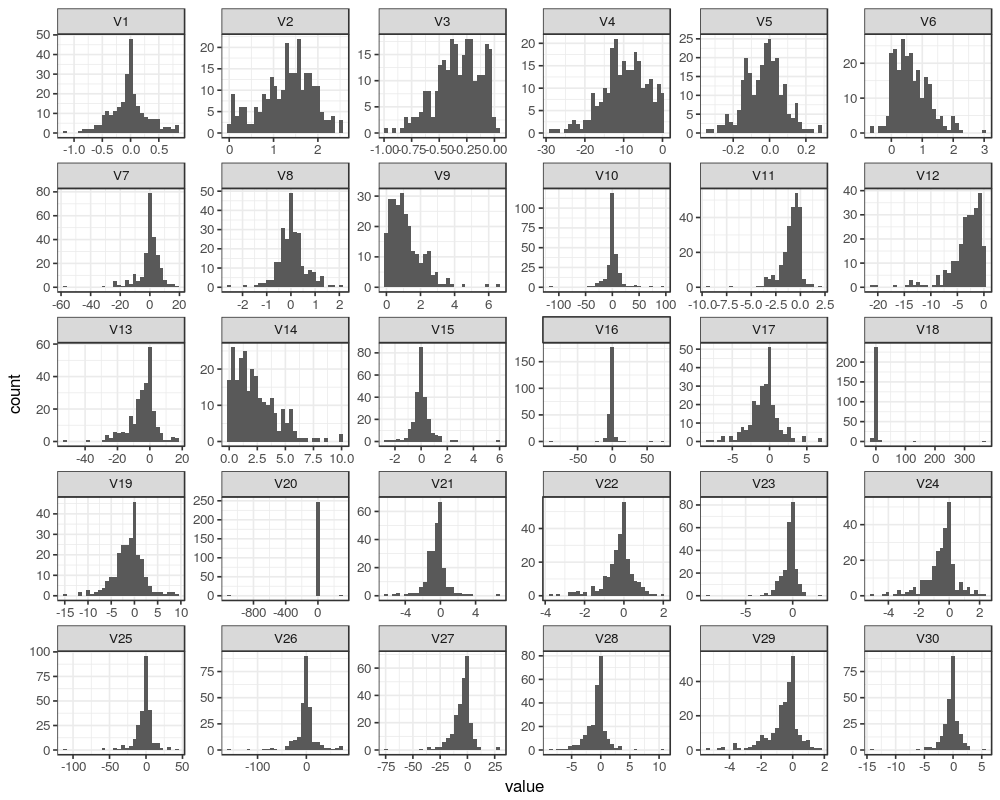
\includegraphics[scale=0.7]{graph53_st_DIRETC_L.png}
\caption{Normalized results of the estimations of the parameters of a Poisson log normal model over 250 runs. The graphs \texttt{V1} to \texttt{V15} represent the regression parameters sorted as follow : at first the three regression parameters for the first observed variable, than for the second up to the fifth. The graphs \texttt{V16} to \texttt{V20} represent the normalized estimation from the variance for each variable of interest. At least, \texttt{V21} to \texttt{V30} represent the covariance sorted as follow : $\sigma_{12}$, $\sigma_{13}$...$\sigma_{15}$, $\sigma_{21}$...$\sigma_{45}$.}
\end{figure}

We see on figure \ref{plot} that the results are not perfect. Some estimators seem to be biased, for other there are outliers very far from the quantity we want to estimate. Our interpretation is that, since we use an algorithm that do not need an explicit expression of the gradient, it sometimes fail to approach the global maximum of the composite pairwise likelihood.
\section{Conclusion}
The Poisson log-normal is a model for count data that allow to perform a linear model, \textit{ie} to estime regression parameters taking in account the dependency structure in the data. We here show that estimating the parameters in maximizing the pairwise composite likelihood provide a consistent estimator as well of the regression parameters, as of the dependency structure (\textit{ie} of the variance and covariance). Furthermore we expect this estimator to be asymptotically normal, which allows to construct confident sets and so to give interpretable results. Finally we looked at the case of a structured dependency matrix. We first expected that the numerical results were easier to interpret, but calculations has to be developped, we failed to get an interpretable expression. At least we performed some simulations of our data. The results are in adequation with what we expected and so support to go further in this sense.\\
\\
At the beginning of the project, the idea was to use the PLN-model to estimate the regression parameters in case of spatially structured data. We first thought that it is as easy as what we developped in section 3, but this case doesn't allow to take in account the covariates. We just give here an insigth and first reflexions on how this model could be adapted to spatial data. \\
Let us recall the general model for estimation of regression parameters. In the more general case we can expect that there are two types of dependency in the data : the dependency between the observed variables, the one we consider in our model, namely $\Sigma$ on the figure \ref{fig} and the dependency between the observations, namely $\Gamma$ on the figure. So there is a variance in the observed variable $V(Y) = \Sigma \otimes \Gamma$. In this report, we assumed repetitions to be independant and identically distributed. In this manner, the $\Gamma$ matrix is diagonal and thus, we only estimate for the $\Gamma$ matrix. In case of spatial data, we have to adapt the PLN-model because we are interested in the case of estimation of the regression parameters with a (spatial)-dependence structure between the repetitions.
\begin{figure}[!h] \label{fig}
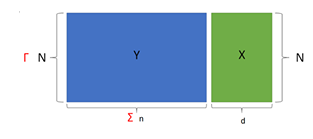
\includegraphics[scale=0.8]{Dependance.png}
\caption{Dependance structured in a data set.We use the notation we previously introduced, namely $n$ the number of variables of interest, $N$ the number of repetitions and $d$ the number of covariates}
\end{figure}

We give here a first description of the model in case of spatial dependency. If we take the notation of figure \ref{fig}, we consider the case were $n=1$, $N$ is the number of sites in the spatial model, and $d$ the number of covariates. In this case, we consider the matrix $\Sigma$ to be diagonal and the matrix $\Gamma$ to be structured. We note $\mathcal{PLN}_s$ the "spatial" PLN model. This model is parametrised by a vector of regression coefficients $\beta \in \mathbb{R}^d$ and the matrix $\Gamma \in \mathcal{M}_N(\mathbb{R})$. We note $(Y^j)_{j \in \{1,...,N\}}$ the observed variable. Let consider a latent vector $Z \sim \mathcal{N}(0,\Gamma)$. Then :
\begin{align*}
Y^j\mid Z^j \sim \mathcal{P}(e^{O+\beta^T X + Z_j})
\end{align*}
We think that also in this case, the estimator constructed by maximizing the pairwise composite likelihood over the pairs is a consistent and assymptotically normal estimator of $\beta$ and $\Gamma$. We propose to investigate also the sparse composite likelihood decribed in \ref{sparse}.\\
\\
At least it is tempting to try to develop a method taking in account both dependency structure. Let note $\mathcal{CL}_o{(M,\Sigma)}=\sum_{j=1}^N \sum_{1 \leq i<k \leq n} \mathrm{log}(Y^j_i, Y^j_k)$ the composite likelihood over the pairs of variables of interest and $\mathcal{CL}_s(M^T,\Gamma) = \sum_{i=1}^n \sum_{1 \leq j<l \leq N} \mathrm{log}(Y^j_i, Y^l_i)$ the composite likelihood over the pairs of observations. We propose that by maximizing the sum of this both likelihoods, \textit{ie} $\mathcal{CL}_o (M, \Sigma) + \mathcal{CL}_s (M^T, \Gamma)$, we construct an consistent and assymptotically normal estimator of the parameters, taking in account for all the dependency structure in a dataset.
\newpage  
\appendix
\section{Appendix} \label{appendix}
\subsection{Gradients} \label{grad}
We calculate the gardient with respect to all the parameters : the regression variables, the variances and covariances. The composite-likelihood is a expressed as a sum over the couples of variables. Since the derivatives are the same for each couple, we performed calculation for one couple; $(j,k)$, for exemple.
\subsubsection{With respect to the regression parameters $M$.}
Let consider $i \in \{1...n\}$. We want to calculate $\partial_{M^{(i)}}\mathrm{log}( h_{(M^{(jk)},\Sigma^{(jk)} \mid X)}(Y_j,Y_k))$.
\begin{align*}
\partial_{M^{(i)}}\mathrm{log}( h_{(M^{(jk)},\Sigma^{(jk)} \mid X)}(Y_j,Y_k)) &= \frac{\partial_{M^{(i)}}h_{(M^{(jk)},\Sigma^{(jk)} \mid X)}(Y_j,Y_k) }{h_{(M^{(jk)},\Sigma^{(jk)} \mid X)}(Y_j,Y_k)}
\end{align*}

Since :
\begin{align*}
\partial_{M^{(i)}}h_{(M^{(jk)},\Sigma^{(jk)} \mid X)}(Y_j,Y_k) &= \mathbb{E}_{(Z_j,Z_k)}[\partial_{M^{(i)}}h_{(M^{(jk)},\Sigma^{(jk)} \mid X)}(Y_j,Y_k \mid Z_j,Z_k)]\\
&= \mathbb{E}_{(Z_j,Z_k)}[\partial_{M^{(i)}}f_{(M^{(jk)},\Sigma^{(jk)} \mid X)}(Y_j\mid Z_j)f_{(M^{(jk)},\Sigma^{(jk)} \mid X)}(Y_k\mid Z_k)]
\end{align*}
if $i \neq j$ and $i \neq k$, this partial derivatives is equal to 0.
Otherwise, taking for example $i=j$, one have :
\begin{align*}
\partial_{M^{(j)}}h_{(M^{(jk)},\Sigma^{(jk)} \mid X)}(Y_j,Y_k) &= &\mathbb{E}_{(Z_j,Z_k)}[\partial_{M^{(j)}}f_{(M^{(jk)},\Sigma^{(jk)} \mid X)}(Y_j\mid Z_j)f_{(M^{(jk)},\Sigma^{(jk)} \mid X)}(Y_k\mid Z_k)]\\
&= &\mathbb{E}_{(Z_j,Z_k)}[ X (Y_j f_{(M^{(jk)},\Sigma^{(jk)} \mid X)} (Y_j \mid Z_j)-(Y_{j}+1) f_{(M^{(jk)},\Sigma^{(jk)} \mid X)}(Y_j+1\mid Z_j))\\
& 	&		 f_{(M^{(jk)},\Sigma^{(jk)} \mid X)}(Y_k\mid Z_k)]\\
&=& X(Y_j h_{(M^{(jk)},\Sigma^{(jk)} \mid X)}(Y_j,Y_k)-(Y_j+1)h_{(M^{(jk)},\Sigma^{(jk)} \mid X)}(Y_j+1,Y_k))
\end{align*}
Where the second equality comes from the fact that $Y_j \mid Z_j$ is following a Poisson-distribution. We have :
\begin{align*}
\partial_{M^{(j)}} h_{M^{(j)},\Sigma^{(jj)} \mid X}(Y_j \mid Z_j) &= \partial_{M^{(j)}} (\mathrm{e}^{Y_j (X^T M^{(j)} + Z_j)} \mathrm{exp}(-e^{X^T M^{(j)} + Z_j}) \frac{1}{Y_j !} )\\
&= X Y_j\frac{\mathrm{e}^{Y_j (X^T M^{(j)} + Z_j)} \mathrm{exp}(-e^{X^T M^{(j)} + Z_j})}{Y_j !} - X \frac{\mathrm{e}^{(Y_j+1) (X^T M^{(j)} + Z_j)} \mathrm{exp}(-e^{X^T M^{(j)} + Z_j})}{Y_j !}\\
&= X(Y_j h_{(M^{(j)},\Sigma^{(jj)} \mid X)} (Y_j \mid Z_j)-(Y_{j}+1) h_{(M^{(j)},\Sigma^{(jj)} \mid X)}(Y_j+1\mid Z_j))
\end{align*}
So we conclude that
\begin{align*}
\partial_{M^{(j)}}\mathrm{log}( h_{(M^{(jk)},\Sigma^{(jk)} \mid X)}(Y_j,Y_k)) &= X(Y_j -(Y_j+1)\frac{H_{(M^{(jk)},\Sigma^{(jk)} \mid X)}(Y_j+1,Y_k)}{h_{(M^{(jk)},\Sigma^{(jk)} \mid X)}(Y_j,Y_k))})
\end{align*}
\subsubsection{With respect to the matrix of variance - covariance.}
The terms of the variance-covariance matrix are only present in the density function of the latent multivariate gaussian distribution. In order to calculate the derivatives we will  follow this path :
\begin{enumerate}
\item We calculate the derivatives of the density function of the bivariate gaussian distribution with respect to the parameters of interest. By derivating under the $\int$ we deduce the derivative of the Poisson-log-normal density function.
\item We integrate by part to have a nice expression of this derivative.
\end{enumerate}
We recall here that the density function of the Poisson log-Normal distribution with regression parameters $M$ and matrix of variance-covariance $\Sigma$, given a vector of covariables $X$ is given by :
\begin{equation*}
h_{(M^{(jk)},\Sigma^{(jk)} \mid X)}(Y_j,Y_k)=\int_{\mathbb{R}^2} f_{e^{X^T M^{(jk)}+z_j}}(Y_j) f_{e^{X^T M^{(jk)}+z_k}}(Y_k) g_{(0,\Sigma^{(jk)})}(z_j,z_k) \mathrm{d}z_j \mathrm{d}z_k
\end{equation*}
With $g_{(0,\Sigma^{(jk)})}$ the density function of the bivariate normale distribution of mean $0$ and variance-covariance $\Sigma^{(jk)}$ and $f_{\beta}$ the density function of a Poisson distribution with parameters $\beta$.
We finally recall that : $g_{(0,\Sigma^{(jk)})}(z_1,z_2)=\frac{1}{2 \pi \sqrt{\mid \sigma_{jj} \sigma_{kk}-\sigma_{jk}^2}\mid} \mathrm{e}^{-\frac{1}{2} \frac{\sigma_{jj} z_1^2 + \sigma_{kk} z_2^2 -2 \sigma_{jk} z_1 z_2}{\sigma_{jj} \sigma_{kk}-\sigma_{jk}^2}}$.

\paragraph{wrt $\sigma_{jj}$ and $\sigma_{kk}$}
\begin{align*}
\partial_{\sigma_{jj}} g_{(0,\Sigma^{(jk)})} (z_1,z_2) &= \frac{1}{2} [ \frac{-\sigma_{kk}}{\sigma_{jj} \sigma_{kk}-\sigma_{jk}^2} +  \frac{(\sigma_{jk} z_1 - \sigma_{kk} z_2)^2}{(\sigma_{jj} \sigma_{kk}-\sigma_{jk}^2)^2}  ]g_{(0,\Sigma^{(jk)})}(z_1,z_2)
\end{align*}

Since the bivariate gaussian distribution admits second order moments, we can apply  the thoerem of derivation under $\int$ and deduce that :
\begin{align*}
\partial_{\sigma_{jj}} h_{(M^{(jk)},\Sigma^{(jk)} \mid X)}(Y_j,Y_k) =\int_{\mathbb{R}^2} & f_{e^{X^T M^{(j)}+z_1}}(Y_j) f_{e^{X^T M^{(k)}+z_2}}(Y_k)\\
&\frac{1}{2} [ \frac{-\sigma_{kk}}{\sigma_{jj} \sigma_{kk}-\sigma_{jk}^2} +  \frac{(\sigma_{jk} z_1 - \sigma_{kk} z_2)^2}{(\sigma_{jj} \sigma_{kk}-\sigma_{jk}^2)^2}  ] g_{(0,\Sigma^{(jk)})}(z_j,z_k) \mathrm{d}z_j \mathrm{d}z_k
\end{align*}

\noindent We will now try to find a nicer expression of this derivative. One can remark that $\partial_{z_2} (-\frac{1}{2} \frac{\sigma_{jj} z_1^2 + \sigma_{kk} z_2^2 -2 \sigma_{jk} z_1 z_2}{\sigma_{jj} \sigma_{kk}-\sigma_{jk}^2}) = \frac{\sigma_{jk} z_1 - \sigma_{kk} z_2}{\sigma_{jj} \sigma_{kk}-\sigma_{jk}^2}$.

This gives the clue to integrate by part with respect to $z_2$. We then have :
\begin{align*}
\partial_{\sigma_{jj}} h_{(M^{(jk)},\Sigma^{(jk)} \mid X)}(Y_j,Y_k) =& \int_{\mathbb{R}} [  f_{e^{X^T M^{(j)}+z_1}}(Y_j) f_{e^{X^T M^{(k)}+z_2}}(Y_k) \frac{\sigma_{jk} z_1 - \sigma_{kk} z_2}{\sigma_{jj} \sigma_{kk}-\sigma_{jk}^2} g_{(0,\Sigma_{jk})}(z_1,z_2) ]_{- \infty}^{+\infty} \mathrm{d}z_1\\
 &- \int_{\mathbb{R}^2} Y_k f_{e^{X^T M^{(j)}+z_1}}(Y_j) f_{e^{X^T M^{(k)}+z_2}}(Y_k) \frac{\sigma_{jk} z_1 - \sigma_{kk} z_2}{\sigma_{jj} \sigma_{kk}-\sigma_{jk}^2} g_{(0,\Sigma_{jk})}(z_1,z_2) \mathrm{d}z_1 \mathrm{d}z_2\\
 &- \int_{\mathbb{R}^2} (Y_k+1) f_{e^{X^T  M^{(j)}+z_1}}(Y_j)  f_{e^{X^T M^{(k)}+z_2}}(Y_k+1) \frac{\sigma_{jk} z_1 - \sigma_{kk} z_2}{\sigma_{jj} \sigma_{kk}-\sigma_{jk}^2} g_{(0,\Sigma_{jk})}(z_1,z_2) \mathrm{d}z_1 \mathrm{d}z_2
\end{align*}
The derivatives of the density function of the Poisson distribution is obtained as we did in the previous section.\\
The first term of this equality is null, so we can again integrate by part wrt $z_2$ and we get :
\begin{align*}
\partial_{\sigma_{jj}} h_{(M^{(jk)},\Sigma^{(jk)} \mid X)}(Y_j,Y_k) &= Y_k^2 h_{(M^{(jk)},\Sigma^{(jk)} \mid X)}(Y_j,Y_k)\\
& - ((Y_k+1)^2 + Y_k (Y_k+1) ) h_{(M^{(jk)},\Sigma^{(jk)} \mid X)}(Y_j,Y_k+1) \\
& + (Y_k+1)(Y_k+2) h_{(M^{(jk)},\Sigma^{(jk)} \mid X)}(Y_j,Y_k+2)
\end{align*} 
We are calculating this gradients in order to approximate the composite log likelihood so we are in fact interested in $\partial_{\sigma_{jj}} \mathrm{log}(h_{(M^{(jk)},\Sigma^{(jk)} \mid X)}(Y_j,Y_k))$, which we now can easily calculate.
\begin{align*}
\partial_{\sigma_{jj}} h_{(M^{(jk)},\Sigma^{(jk)} \mid X)}(Y_j,Y_k) &= Y_k^2 - ((Y_k+1)^2 + Y_k (Y_k+1) ) \frac{h_{(M^{(jk)},\Sigma^{(jk)} \mid X)}(Y_j,Y_k+1) } {h_{(M^{(jk)},\Sigma^{(jk)} \mid X)}(Y_j,Y_k)}\\
& + (Y_k+1)(Y_k+2)\frac{ h_{(M^{(jk)},\Sigma^{(jk)} \mid X)}(Y_j,Y_k+2)}{h_{(M^{(jk)},\Sigma^{(jk)} \mid X)}(Y_j,Y_k)}
\end{align*}
Symetrically we have with respect to $\sigma_{kk}$ :
\begin{align*}
\partial_{\sigma_{kk}} h_{(M^{(jk)},\Sigma^{(jk)} \mid X)}(Y_j,Y_k) &= Y_j^2 - ((Y_j+1)^2 + Y_j (Y_j+1) ) \frac{h_{(M^{(jk)},\Sigma^{(jk)} \mid X)}(Y_j+1,Y_k) } {h_{(M^{(jk)},\Sigma^{(jk)} \mid X)}(Y_j,Y_k)}\\
& + (Y_j+1)(Y_j+2)\frac{ h_{(M^{(jk)},\Sigma^{(jk)} \mid X)}(Y_j+2,Y_k)}{h_{(M^{(jk)},\Sigma^{(jk)} \mid X)}(Y_j,Y_k)}
\end{align*}

\paragraph{with respect to $\sigma_{jk}$ :}
\begin{align*}
\partial_{\sigma_{jk}}g_{(0,\Sigma^{(jk)})}(z_1,z_2) &= [\frac{\sigma_{jk}}{\sigma_{jj} \sigma_{kk} - \sigma_{jk}^2} + \frac{-\sigma_{jk} ( \sigma_{jj} z_1^2 + \sigma_{kk} z_2^2 ) + \sigma_{jk} z_1 z_2 + \sigma_{jj} \sigma_{kk} z_1 z_2}{(\sigma_{jj} \sigma_{kk} - \sigma_{jk}^2)^2}] g_{(0,\Sigma^{(jk)})}(z_1,z_2)
\end{align*}
Again we can apply the theorem of derivating under the $\int$. We deduce that :
\begin{align*}
&\partial_{\sigma_{jk}} h_{(M^{(jk)},\Sigma^{(jk)} \mid X)}(Y_j,Y_k) =
\int_{\mathbb{R}^2} f_{e^{X^T M^{(j)}+z_1}}(Y_j) f_{e^{X^T M^{(k)}+z_2}}(Y_k)\\
&[   \frac{\sigma_{jk}}{\sigma_{jj} \sigma_{kk} - \sigma_{jk}^2} + \frac{-\sigma_{jk} ( \sigma_{jj} z_1^2 + \sigma_{kk} z_2^2 ) + \sigma_{jk} z_1 z_2 + \sigma_{jj} \sigma_{kk} z_1 z_2}{(\sigma_{jj} \sigma_{kk} - \sigma_{jk}^2)^2}] g_{(0,\Sigma^{(jk)})}(z_1,z_2) \mathrm{d}z_1 \mathrm{d}z_2
\end{align*}

One can note that :
\begin{align*}
\partial_{z_1} ( - \frac{1}{2} \frac{\sigma_{jj} z_1^2 + \sigma_{kk} z_2^2 - 2 \sigma_{jk} z_1 z_2 }{\sigma_{jj} \sigma_{kk}-  \sigma_{jk}^2} ) & \partial_{z_2} ( - \frac{1}{2} \frac{\sigma_{jj} z_1^2 + \sigma_{kk} z_2^2 - 2 \sigma_{jk} z_1 z_2 }{\sigma_{jj} \sigma_{kk}-  \sigma_{jk}^2} ) =\\
&  \frac{-\sigma_{jk} ( \sigma_{jj} z_1^2 + \sigma_{kk} z_2^2 ) + \sigma_{jk} z_1 z_2 + \sigma_{jj} \sigma_{kk} z_1 z_2}{(\sigma_{jj} \sigma_{kk} - \sigma_{jk}^2)^2}
\end{align*}
Which gives a clue that we could do again two integrations by part : one towards $z_1$ and one towards $z_2$. \\
We will do a first integration by part with respect to $z_1$. We note that : $ \partial_{z_1} ( \frac{\sigma_{jk}z_1-\sigma_{kk}z_2}{\sigma_{jj} \sigma_{kk}- \sigma_{jk}^2} g_{(0,\Sigma^{(jk)})}(z_1,z_2) = [\frac{\sigma_{jk}}{\sigma_{jj} \sigma_{kk} - \sigma_{jk}^2} + \frac{-\sigma_{jk} ( \sigma_{jj} z_1^2 + \sigma_{kk} z_2^2 ) + \sigma_{jk} z_1 z_2 + \sigma_{jj} \sigma_{kk} z_1 z_2}{(\sigma_{jj} \sigma_{kk} - \sigma_{jk}^2)^2}] g_{(0,\Sigma^{(jk)})}(z_1,z_2)$. And taking the derivative of the Poisson density function with respect to its parameters allows us to conclude that :
\begin{align*}
&\partial_{\sigma_{jk}}h_{(M^{(jk)},\Sigma^{(jk)} \mid X)}(Y_j,Y_k) = \int_{\mathbb{R}} [ f_{e^{X^T M^{(j)}+z_1}}(Y_j) f_{e^{X^T M^{(k)}+z_2}}(Y_k) \frac{\sigma_{jk}z_1-\sigma_{kk}z_2}{\sigma_{jj} \sigma_{kk}- \sigma_{jk}^2} g_{(0,\Sigma^{(jk)})}(z_1,z_2)]_{- \infty}^{+ \infty} \mathrm{d}z_2\\
& - \int_{\mathbb{R}^2} (Y_j f_{e^{X^T M^{(j)}+z_1}}(Y_j)- (Y_j+1) f_{e^{X^T M^{(j)}+z_1}}(Y_j+1)) f_{e^{X^T M^{(k)}+z_2}}(Y_k) \frac{\sigma_{jk} z_1 - \sigma_{kk} z_2}{\sigma_{jj} \sigma_{kk} - \sigma_{jk}^2} g_{(0,\Sigma^{(jk)})}(z_1,z_2) \mathrm{d}z_1  \mathrm{d}z_2
\end{align*}
The first right-hand term of the equality being equal to zero, we have, integrating by part again but this time wrt $z_2$, we have :
\begin{align*}
&\partial_{\sigma_{jk}}h_{(M^{(jk)},\Sigma^{(jk)} \mid X)}(Y_j,Y_k) =\int_{\mathbb{R}^2} (Y_j f_{e^{X^T M^{(jk)}+z_1}}(Y_j)- (Y_j+1) f_{e^{X^T M^{(j)}+z_1}}(Y_j+1))\\
& (Y_k f_{e^{X^T M^{(k)}+z_2}}(Y_k)-(Y_k + 1) f_{e^{X^T M^{(jk)}+z_2}}(Y_k+1))  g_{(0,\Sigma^{(jk)})}(z_1,z_2) \mathrm{d}z_1  \mathrm{d}z_2
\end{align*}
What we can also write :
\begin{align*}
\partial_{\sigma_{jk}}h_{(M^{(jk)},\Sigma^{(jk)} \mid X)}(Y_j,Y_k) = &Y_k Y_j h_{(M^{(jk)},\Sigma^{(jk)} \mid X)}(Y_j,Y_k)-(Y_k+1)Y_j h_{(M^{(jk)},\Sigma^{(jk)} \mid X)}(Y_j,Y_k+1)\\
& -(Y_j+1)Y_k h_{(M^{(jk)},\Sigma^{(jk)} \mid X)}(Y_j,Y_k)+ (Y_k+1) (Y_j+1)h_{(M^{(jk)},\Sigma^{(jk)} \mid X)}(Y_j+1,Y_k+1))
\end{align*}
Again we are interested in $\partial_{\sigma_{jk}}\mathrm{log}h_{(M^{(jk)},\Sigma^{(jk)} \mid X)}(Y_j,Y_k)$ which we can now easily calculate by dividing the above quantity by $h_{(M^{(jk)},\Sigma^{(jk)} \mid X)}(Y_j,Y_k)$.

\subsection{Hessian}
We have seen that we expect our estimators to be assymptotically normal with matrix of variance-covariance : 
\begin{center}
$(\mathbb{E}_{Y_1...Y_n} \partial^2_{(M,\Sigma)} \mathcal{CL}(M^\ast, \Sigma^\ast))^{-1} \mathbb{E}_{Y_1...Y_n} [\partial_{(M,\Sigma)} \mathcal{CL}(M^\ast, \Sigma^\ast) (\partial_{(M,\Sigma)} \mathcal{CL}(M^\ast, \Sigma^\ast))^T](\mathbb{E}_{Y_1...Y_n} \partial^2_{(M,\Sigma)} \mathcal{CL}(M^\ast, \Sigma^\ast))^{-1}$
\end{center} 
In practice, we want to estimate this quantity by the empirical mean over the repetitions in order to calculate confident sets. Thus we need to explicitly calculate the second derivatives .
\begin{landscape}
\paragraph{$\partial^2 M^{(i)}$}
\begin{align*}
\partial^2 _{ M^{(i)}} \mathcal{CL}_{(Y_1,...,Y_n,O)}(M,\Sigma \mid X) =& X X^T \sum_{j \neq i} \frac{1}{h_{(M^{(ij)},\Sigma^{(ij)} \mid X)}(Y_i,Y_j)^2} [(Y_i+1)(Y_i+2)h_{(M^{(ij)},\Sigma^{(ij)} \mid X)}(Y_i,Y_j)h_{(M^{(ij)},\Sigma^{(ij)} \mid X)}(Y_i+2,Y_j)\\& - (Y_i+1)h_{(M^{(ij)},\Sigma^{(ij)} \mid X)}(Y_i,Y_j)h_{(M^{(ij)},\Sigma^{(ij)} \mid X)}(Y_i+1,Y_j)-(Y_i+1)^2 h_{(M^{(ij)},\Sigma^{(ij)} \mid X)}(Y_i+1,Y_j)^2] 
\end{align*}
\paragraph{$\partial M^{(j)} \partial M^{(i)}$ ($i \neq j$)}
\begin{align*}
\partial^2 _{M^{(i)} M^{(j)}} \mathcal{CL}_{(Y_1,...,Y_n,O)}(M,\Sigma \mid X) =& X X^T \frac{(Y_i+1)(Y_j+1)}{h_{(M^{(ij)},\Sigma^{(ij)} \mid X)}(Y_i,Y_j)^2} \\
&[h_{(M^{(ij)},\Sigma^{(ij)} \mid X)}(Y_i+1,Y_j+1)h_{(M^{(ij)},\Sigma^{(ij)} \mid X)}(Y_i,Y_j) - h_{(M^{(ij)},\Sigma^{(ij)} \mid X)}(Y_i+1,Y_j)h_{(M^{(ij)},\Sigma^{(ij)} \mid X)}(Y_i,Y_j+1)]
\end{align*}
\paragraph{$\partial^2 \sigma_{ii}$}
\begin{align*}
\partial^2_{ \sigma_{ii}}\mathcal{CL}_{(Y_1,...,Y_n,O)}(M,\Sigma \mid X) =  \sum_{j \neq i} & \frac{(Y_j+1)}{h_{(M^{(ij)},\Sigma^{(ij)} \mid X)}(Y_i,Y_j)^2} [ -(2 Y_j+1)^2 h_{(M^{(ij)},\Sigma^{(ij)} \mid X)}(Y_i,Y_j+1)h_{(M^{(ij)},\Sigma^{(ij)} \mid X)}(Y_i,Y_j)\\
&+(Y_j+2) (4 Y_j^2 + 12 Y_j +7) h_{(M^{(ij)},\Sigma^{(ij)} \mid X)}(Y_i,Y_j+2) h_{(M^{(ij)},\Sigma^{(ij)} \mid X)}(Y_i,Y_j)\\
&- 2 (Y_j+2)(Y_j+3)(2 Y_j+3) h_{(M^{(ij)},\Sigma^{(ij)} \mid X)}(Y_i,Y_j+3)h_{(M^{(ij)},\Sigma^{(ij)} \mid X)}(Y_i,Y_j)\\
& -(2 Y_j+1)^2 (Y_j+1) h_{(M^{(ij)},\Sigma^{(ij)} \mid X)}(Y_i,Y_j+1)^2\\
& + 2(Y_j+1)(Y_j+2)(2Y_j+1)h_{(M^{(ij)},\Sigma^{(ij)} \mid X)}(Y_i,Y_j+2)h_{(M^{(ij)},\Sigma^{(ij)} \mid X)}(Y_i,Y_j+1)\\
&+(Y_j+2)(Y_j+3)(Y_j+4)h_{(M^{(ij)},\Sigma^{(ij)} \mid X)}(Y_i,Y_j+4)h_{(M^{(ij)},\Sigma^{(ij)} \mid X)}(Y_i,Y_j)\\
&-(Y_j+2)^2(Y_j+1)h_{(M^{(ij)},\Sigma^{(ij)} \mid X)}(Y_i,Y_j+2)^2]
\end{align*}
\paragraph{$\partial^2 \sigma_{ii} \sigma_{jj}$ ($i \neq j$}
\begin{align*}
\partial^2_{\sigma_{ii} \sigma_{jj}} \mathcal{CL}_{(Y^1,...,Y^n,O)}(M,\Sigma \mid X) = & \frac{(Y_j+1)(Y_i+1)}{h_{(M^{(ij)},\Sigma^{(ij)} \mid X)}(Y_i,Y_j)^2} [(2Y_i+1) [ (2Y_j+1) (h_{(M^{(ij)},\Sigma^{(ij)} \mid X)}(Y_i+1,Y_j+1)h_{(M^{(ij)},\Sigma^{(ij)} \mid X)}(Y_i,Y_j)\\
& - h_{(M^{(ij)},\Sigma^{(ij)} \mid X)}(Y_i+1,Y_j)h_{(M^{(ij)},\Sigma^{(ij)} \mid X)}(Y_i,Y_j+1) )\\
& + (Y_j+2) (h_{(M^{(ij)},\Sigma^{(ij)} \mid X)}(Y_i,Y_j+2)h_{(M^{(ij)},\Sigma^{(ij)} \mid X)}(Y_i+1,Y_j)- h_{(M^{(ij)},\Sigma^{(ij)} \mid X)}(Y_i,Y_j)h_{(M^{(ij)},\Sigma^{(ij)} \mid X)}(Y_i+1,Y_j+2) )]\\
& + (Y_i+2) [ (2Y_j+1) h_{(M^{(ij)},\Sigma^{(ij)} \mid X)}(Y_i,Y_j+1)h_{(M^{(ij)},\Sigma^{(ij)} \mid X)}(Y_i+2,Y_j)-h_{(M^{(ij)},\Sigma^{(ij)} \mid X)}(Y_i+2,Y_j+2)h_{(M^{(ij)},\Sigma^{(ij)} \mid X)}(Y_i,Y_j) )\\
& +(Y_j+2) ( h_{(M^{(ij)},\Sigma^{(ij)} \mid X)}(Y_i,Y_j) h_{(M^{(ij)},\Sigma^{(ij)} \mid X)}(Y_i+2,Y_j+2)-h_{(M^{(ij)},\Sigma^{(ij)} \mid X)}(Y_i,Y_j+2)h_{(M^{(ij)},\Sigma^{(ij)} \mid X)}(Y_i+2,Y_j) ) ] ]
\end{align*}
\paragraph{$\partial \sigma_{ii} M^{(i)}$}
\begin{align*}
\partial^2_{ \sigma_{ii} M^{(i)}} \mathcal{CL}_{(Y^1,...,Y^n,O)}(M,\Sigma \mid X) =  X \sum_{j \neq i} & \frac{(Y_i+1)(Y_j+1)}{h_{(M^{(ij)},\Sigma^{(ij)} \mid X)}(Y_i,Y_j)^2} [(2Y_j+1) (h_{(M^{(ij)},\Sigma^{(ij)} \mid X)}(Y_i+1,Y_j+1)h_{(M^{(ij)},\Sigma^{(ij)} \mid X)}(Y_i,Y_j)\\
&-h_{(M^{(ij)},\Sigma^{(ij)} \mid X)}(Y_i,Y_j+1)h_{(M^{(ij)},\Sigma^{(ij)} \mid X)}(Y_i+1,Y_j)) + (Y_j+2) (h_{(M^{(ij)},\Sigma^{(ij)} \mid X)}(Y_i,Y_j+2)h_{(M^{(ij)},\Sigma^{(ij)} \mid X)}(Y_i+1,Y_j)\\
&-h_{(M^{(ij)},\Sigma^{(ij)} \mid X)}(Y_i+1,Y_j+2)h_{(M^{(ij)},\Sigma^{(ij)} \mid X)}(Y_i,Y_j) ) ]
\end{align*}
\paragraph{$\partial \sigma_{ii} M^{(j)}$ ($i \neq j$)}
\begin{align*}
\partial^2 _{\sigma_{ii} M^{(j)} } \mathcal{CL}_{(Y^1,...,Y^n,O)}(M,\Sigma \mid X) =& X \frac{(Y_j+1)}{h_{(M^{(ij)},\Sigma^{(ij)} \mid X)}(Y_i,Y_j)^2}\\
&[-(2Y_j+1) h_{(M^{(ij)},\Sigma^{(ij)} \mid X)}(Y_i,Y_j+1)h_{(M^{(ij)},\Sigma^{(ij)} \mid X)}(Y_i,Y_j)\\
& + (Y_j+2)h_{(M^{(ij)},\Sigma^{(ij)} \mid X)}(Y_i,Y_j) [(2Y_j+3)h_{(M^{(ij)},\Sigma^{(ij)} \mid X)}(Y_i,Y_j+2)-(Y_j+3) h_{(M^{(ij)},\Sigma^{(ij)} \mid X)}(Y_i,Y_j+3)] \\
&+ (Y_j+1) h_{(M^{(ij)},\Sigma^{(ij)} \mid X)}(Y_i,Y_j+1)[(Y_j+2)h_{(M^{(ij)},\Sigma^{(ij)} \mid X)}(Y_i,Y_j+2)-(2Y_j+1)h_{(M^{(ij)},\Sigma^{(ij)} \mid X)}(Y_i,Y_j+1)]]
\end{align*}
\paragraph{$\partial^2\sigma_{ij}$}
\begin{align*}
\partial^2 _{\sigma_{ij}}  \mathcal{CL}_{(Y^1,...,Y^n,O)}(M,\Sigma \mid X) =& \frac{4}{h_{(M^{(ij)},\Sigma^{(ij)} \mid X)}(Y_i,Y_j)^2}\\
&[-(Y_j)^2(Y_j+1)h_{(M^{(ij)},\Sigma^{(ij)} \mid X)}(Y_i,Y_j+1)h_{(M^{(ij)},\Sigma^{(ij)} \mid X)}(Y_i,Y_j)\\
&+(Y_i+1)(Y_j+1)(2Y_iY_k+2Y_i+2Y_j+1)h_{(M^{(ij)},\Sigma^{(ij)} \mid X)}(Y_i+1,Y_j+1)h_{(M^{(ij)},\Sigma^{(ij)} \mid X)}(Y_i,Y_j)\\
&+(Y_i)^2(Y_j+1)(Y_j+2)h_{(M^{(ij)},\Sigma^{(ij)} \mid X)}(Y_i,Y_j+2)h_{(M^{(ij)},\Sigma^{(ij)} \mid X)}(Y_i,Y_j)\\
&-(Y_j+1)(Y_j+2)(Y_i+1)(2Y_i+1)h_{(M^{(ij)},\Sigma^{(ij)} \mid X)}(Y_i+1,Y_j+2)h_{(M^{(ij)},\Sigma^{(ij)} \mid X)}(Y_i,Y_j)\\
&-Y_i^2(Y_j+1)^2 h_{(M^{(ij)},\Sigma^{(ij)} \mid X)}(Y_i,Y_j+1)^2 - 2 Y_iY_j(Y_i+1-Y_j+1)h_{(M^{(ij)},\Sigma^{(ij)} \mid X)}(Y_i,Y_j+1)h_{(M^{(ij)},\Sigma^{(ij)} \mid X)}(Y_i+1,Y_j)\\
&+2 Y_i (Y_j+1)^2(Y_i+1)h_{(M^{(ij)},\Sigma^{(ij)} \mid X)}(Y_i+1,Y_j+1)h_{(M^{(ij)},\Sigma^{(ij)} \mid X)}(Y_i,Y_j+1)\\
&-Y_j^2(Y_k+1)h_{(M^{(ij)},\Sigma^{(ij)} \mid X)}(Y_i+1,Y_j)h_{(M^{(ij)},\Sigma^{(ij)} \mid X)}(Y_i,Y_j)\\
&+Y_j^2(Y_i+1)(Y_i+2)h_{(M^{(ij)},\Sigma^{(ij)} \mid X)}(Y_i+2,Y_j)h_{(M^{(ij)},\Sigma^{(ij)} \mid X)}(Y_i,Y_j)-(Y_i+1)^2Y_j^2 h_{(M^{(ij)},\Sigma^{(ij)} \mid X)}(Y_i+1,Y_j)^2\\
&+2(Y_i+1)^2Y_j(Y_j+1)h_{(M^{(ij)},\Sigma^{(ij)} \mid X)}(Y_i+1,Y_j+1)h_{(M^{(ij)},\Sigma^{(ij)} \mid X)}(Y_i+1,Y_j)\\
&-(Y_i+1)(Y_j+1)(Y_i+2)(2Y_j+1)h_{(M^{(ij)},\Sigma^{(ij)} \mid X)}(Y_i+2,Y_j+1)h_{(M^{(ij)},\Sigma^{(ij)} \mid X)}(Y_i,Y_j)\\
&(Y_i+1)(Y_i+2)(Y_j+1)(Y_j+2)h_{(M^{(ij)},\Sigma^{(ij)} \mid X)}(Y_i+2,Y_j+2)h_{(M^{(ij)},\Sigma^{(ij)} \mid X)}(Y_i,Y_j)-(Y_i+1)^2(Y_j+1)^2h_{(M^{(ij)},\Sigma^{(ij)} \mid X)}(Y_i+1,Y_j+1)^2
\end{align*}
\paragraph{$\partial^2 M^{(i)} \sigma_{ij}$}
\begin{align*}
\partial^2_{M^{(i)} \sigma_{ij}}  \mathcal{CL}_{(Y^1,...,Y^n,O)}(M,\Sigma \mid X) =& 2 X \frac{(Y_i+1)}{h_{(M^{(ij)},\Sigma^{(ij)} \mid X)}(Y_i,Y_j)^2} [ h_{(M^{(ij)},\Sigma^{(ij)} \mid X)}(Y_i,Y_j) ((Y_j+1) (Y_i+1) h_{(M^{(ij)},\Sigma^{(ij)} \mid X)}(Y_i+1,Y_j+1) - Y_j h_{(M^{(ij)},\Sigma^{(ij)} \mid X)}(Y_i+1,Y_j)\\
&+(Y_i+2)Y_j h_{(M^{(ij)},\Sigma^{(ij)} \mid X)}(Y_i+2,Y_j) - (Y_j+1)(Y_i+2)h_{(M^{(ij)},\Sigma^{(ij)} \mid X)}(Y_i+2,Y_j+1))\\
& + h_{(M^{(ij)},\Sigma^{(ij)} \mid X)}(Y_i+1,Y_j)(-Y_i(Y_j+1) h_{(M^{(ij)},\Sigma^{(ij)} \mid X)}(Y_i,Y_j+1)-Y_j (Y_i+1) h_{(M^{(ij)},\Sigma^{(ij)} \mid X)}(Y_i+1,Y_j)\\
&+(Y_j+1)(Y_i+1)h_{(M^{(ij)},\Sigma^{(ij)} \mid X)}(Y_i+1,Y_j+1))]
\end{align*}
\paragraph{$\partial^2 \sigma{ij} \sigma{ii}$}
\begin{align*}
\partial^2_{ \sigma_{ii} \sigma_{ij}}  \mathcal{CL}_{(Y^1,...,Y^n,O)}(M,\Sigma \mid X) =&\frac{2 (Y_j+1)}{h_{(M^{(ij)},\Sigma^{(ij)} \mid X)}(Y_i,Y_j)^2}[h_{(M^{(ij)},\Sigma^{(ij)} \mid X)}(Y_i,Y_j)\\
&((Y_i+1)(2Y_j+1)(Y_j+1)h_{(M^{(ij)},\Sigma^{(ij)} \mid X)}(Y_i+1,Y_j+1)-3(Y_i+1)(Y_j+1)(Y_j+2)h_{(M^{(ij)},\Sigma^{(ij)} \mid X)}(Y_i+1,Y_j+2)\\
&-Y_i(2Y_j+1)h_{(M^{(ij)},\Sigma^{(ij)} \mid X)}(Y_i,Y_j+1)+Y_i(2Y_j+3)(Y_j+2)h_{(M^{(ij)},\Sigma^{(ij)} \mid X)}(Y_i,Y_j+2)\\
&-Y_i(Y_j+2)(Y_j+3)h_{(M^{(ij)},\Sigma^{(ij)} \mid X)}(Y_i,Y_j+3)+(Y_i+1)(Y_j+2)(Y_j+3)h_{(M^{(ij)},\Sigma^{(ij)} \mid X)}(Y_i+1,Y_j+3))\\
&+(Y_j(Y_i+1)h_{(M^{(ij)},\Sigma^{(ij)} \mid X)}(Y_i+1,Y_j)+Y_i(Y_j+1)h_{(M^{(ij)},\Sigma^{(ij)} \mid X)}(Y_i,Y_j+1)-(Y_j+1)(Y_i+1)h_{(M^{(ij)},\Sigma^{(ij)} \mid X)}(Y_i+1,Y_j+1))\\
&((Y_j+2)h_{(M^{(ij)},\Sigma^{(ij)} \mid X)}(Y_i,Y_j+2)-(2Y_j+1)h_{(M^{(ij)},\Sigma^{(ij)} \mid X)}(Y_i,Y_j+1))]
\end{align*}
\end{landscape}

\subsection{Spatial gradient and hessian} \label{spatial}
We just expose here the first steps of calculation of the gradient in case of a structured dependency. Calculation didn't end up. We propose to try again using the Mahalanobis metrix.\\
Since calculation of the gradient of the desity function of the bivariate Poisson log-normal distribution is independent of the couple of observation choosen, we consider one couple of variables, $(Y_i,Y_j)$ for example. The density of the PLN for $(Y_1,Y_2)$ is given by :
\begin{align*}
h_{(M^{(ij)},\sigma^2,\alpha \mid X)}(Y_i,Y_j) = \int \int _{\mathbb{R}^2} f_{(e^{X^T M^{(i)} + z_i})}(Y_i) f_{(e^{X^T M^{(j)} + z_j})}(Y_j) \frac{1}{2 \pi \sigma^2 \sqrt{1-e^{-2 \alpha d_{ij}}}} e^{- \frac{z_i^2+z_j^2-2 e^{- \alpha d_{ij}} z_i z_j}{2 \sigma^2 (1- e^{-2 \alpha d_{ij}})}} \mathrm{d}z_i \mathrm{d} z_j
\end{align*}
With $f_{(e^{X^T M^{(i)} + z_i})}(Y_i)$ the density function of a Poisson-law with parameter $e^{X^T M^{(i)} + z_i}$ taken in $Y_1$.\\
\\
\paragraph{Gradient with respect to $\sigma^2$}
Derivating under $\int \int$, one have :
\begin{align*}
\partial_{\sigma^2} h_{(M^{(ij)},\sigma^2,\alpha \mid X)}(Y_i,Y_j) =\int \int _{\mathbb{R}^2} & f_{(e^{X^T M^{(i)} + z_i})}(Y_i) f_{(e^{X^T M^{(j)} + z_j})}(Y_j) \\
&[-\frac{1}{\sigma^2} + \frac{1}{2} \frac{z_i^2 + z_j^2 - 2 e^{- \alpha d_{ij}} z_i z_j}{(\sigma^2)^2 (1-e^{-2 \alpha d_ij})}] \\
& \frac{1}{2 \pi \sigma^2 \sqrt{1-e^{-2 \alpha d_{ij}}}} e^{- \frac{z_i^2+z_j^2-2 e^{- \alpha d_{ij}} z_i z_j}{2 \sigma^2 (1- e^{-2 \alpha d_{ij}})}} \mathrm{d}z_i \mathrm{d} z_j
\end{align*}
 So we have :
 \begin{align*}
 \partial_{\sigma^2} h_{(M^{(ij)},\sigma^2,\alpha \mid X)}(Y_i,Y_j) = -\frac{1}{\sigma^2}h_{(M^{(ij)},\sigma^2,\alpha \mid X)}(Y_i,Y_j)  \\
  - \int \int_{\mathbb{R}^2} f_{(e^{X^T M^{(i)} + z_i})}(Y_i) f_{(e^{X^T M^{(j)} + z_j})}(Y_j) z_i \partial_{z_i} (- \frac{z_i^2+z_j^2-2 e^{- \alpha d_{ij}} z_i z_j}{2 \sigma^2 (1- e^{-2 \alpha d_{ij}}}) \frac{e^{- \frac{z_i^2+z_j^2-2 e^{- \alpha d_{ij}} z_i z_j}{2 \sigma^2 (1- e^{-2 \alpha d_{ij}})}}}{2 \pi \sigma^2 \sqrt{1-e^{-2 \alpha d_{ij}}}}  \mathrm{d}z_i \mathrm{d} z_j \\
 - \int \int_{\mathbb{R}^2} f_{(e^{X^T M^{(i)} + z_i})}(Y_i) f_{(e^{X^T M^{(j)} + z_j})}(Y_j) z_j \partial_{z_j} (- \frac{z_i^2+z_j^2-2 e^{- \alpha d_{ij}} z_i z_j}{2 \sigma^2 (1- e^{-2 \alpha d_{ij}}}) \frac{e^{- \frac{z_i^2+z_j^2-2 e^{- \alpha d_{ij}} z_i z_j}{2 \sigma^2 (1- e^{-2 \alpha d_{ij}})}}}{2 \pi \sigma^2 \sqrt{1-e^{-2 \alpha d_{ij}}}}  \mathrm{d}z_i \mathrm{d} z_j
 \end{align*}
 From here the idea is to integrate by part the two last terms. \\
 We intergrate $\partial_{z_j} (- \frac{z_i^2+z_j^2-2 e^{- \alpha d_{ij}} z_i z_j}{2 \sigma^2 (1- e^{-2 \alpha d_{ij}}}) \frac{1}{2 \pi \sigma^2 \sqrt{1-e^{-2 \alpha d_{ij}}}} e^{- \frac{z_i^2+z_j^2-2 e^{- \alpha d_{ij}} z_i z_j}{2 \sigma^2 (1- e^{-2 \alpha d_{ij}})}}$ and derive $ z_j f_{(e^{M^{(i)} X + z_i})}(Y_i) f_{(e^{M^{(j)} X + z_j})}(Y_j)$ with respect to $z_j$. If we note $g_{(\alpha, \sigma^2)}(z_i,z_j) =  \frac{e^{- \frac{z_i^2+z_j^2-2 e^{- \alpha d_{ij}} z_i z_j}{2 \sigma^2 (1- e^{-2 \alpha d_{ij}})}}}{2 \pi \sigma^2 \sqrt{1-e^{-2 \alpha d_{ij}}}} $, we then get :
 \begin{align*}
 - \int \int_{\mathbb{R}^2} f_{(e^{M^{(i)} X + z_i})}(Y_i) f_{(e^{M^{(j)} X + z_j})}(Y_j) z_j \partial_{z_j} (- \frac{z_i^2+z_j^2-2 e^{- \alpha d_{ij}} z_i z_j}{2 \sigma^2 (1- e^{-2 \alpha d_{ij}}}) g_{(\alpha,\sigma^2)} (z_i,z_j) \mathrm{d}z_i \mathrm{d} z_j\\
 = h_{(M^{(ij)},\sigma^2,\alpha \mid X)}
  +  \int \int z_j(Y_j f_{(e^{M^{(j)} X + z_j})}(Y_j) - (Y_j+1) f_{(e^{M^{(j)} X + z_j})}(Y_j+1))g_{(\alpha,\sigma^2)} (z_i,z_j) \mathrm{d}z_i \mathrm{d} z_j
 \end{align*}
We are not able to estime this quantity and so stopped here our calculations.
\bibliographystyle{plain}
\bibliography{Biblio.bib}
\end{document}